\section{Network Operating System Vs Distributed Operating System}
\begin{table}[H]
    \renewcommand\arraystretch{1.1}
    \hspace{-2cm}
    \begin{tabular}{p{3cm}|p{7cm}|p{7cm}}
         \textbf{Parameter} & \textbf{Network Operating System} & \textbf{Distributed Operating System} 
         \\ \hline \hline
         Definition
         & The network operating system is the platform to run a system software on a server and allow the server to manage the users, data, groups, security, applications and other networking functions. It is considered as the primary form of an operating system for the distributed architecture. The idea behind the network operating system is to permit resource sharing among two or more computers operating under their own OSs.
         & The distributed operating system handles a group of independent computers and makes them look like an ordinary centralised operating system. This is achieved by enabling the proper communication between the different computers connected with each other. The main aim of the distributed operating system is the transparency where the use of multiple hardware resources is hidden from the users. The distributed operating system is less autonomous than network operating system as the system has complete control in this environment.
         \\ \hline
         Objective 
         & Provision of local services to the remote client.
         & Management of hardware resource.
         \\ \hline
         Use 
         & Loosely coupled system employed in heterogeneous computers.
         & Tightly coupled system used in multiprocessor and homogeneous computers.
         \\ \hline
         Architecture 
         & 2-tier client/server architecture.
         & N-tier client/server architecture.
         \\ \hline
         Level of transparency  
         & Low
         & High
         \\ \hline
         Basis for communication 
         & Files
         & Shared memory and messages
         \\ \hline
         Resource Management 
         & Handled at each node.
         & Global central or distributed management.
         \\ \hline
         Implementation Complexity
         & Easy
         & Hard
         \\ \hline
         Scalability 
         & High
         & Less/moderate
         \\ \hline
         Openness 
         & Open
         & Closed
         \\ \hline
         Operating system on all nodes 
         & Can be different
         & Same
         \\ \hline
         Rate of autonomy  
         & High
         & Low
         \\ \hline
         Fault tolerance
         & Less
         & High
         \\ \hline
    \end{tabular}
    \caption{Network Operating System Vs Distributed Operating System}
    \label{tab:NetworkOSvsDistributedOS}
\end{table}

% \begin{figure}[H]
%     \centering
%     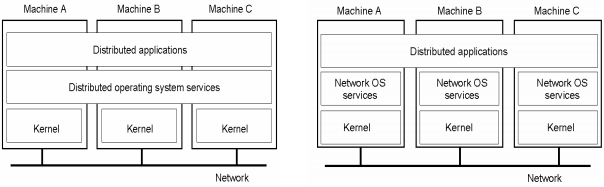
\includegraphics[width=\textwidth]{assets/distributed-operating-system}
%     \caption{Basic architecture of Distributed Operating System and Network Operating System}
%     \label{fig:NetworkOSvsDistributedOS}
% \end{figure}